% Created 2016-08-17 Wed 14:38
\documentclass[tikz]{standalone}

\usepackage[utf8]{inputenc}
\usepackage[T1]{fontenc}

\usepackage{circledsteps}

\RequirePackage{xcolor}

%% HPI color definitions according to the design manual
% These do not exactly match the RGB values used in the Powerpoint slide master due to unknown reasons
\definecolor{hpiyellow}{RGB}{246,168,0}
\definecolor{hpiorange}{RGB}{221,97,8}
\definecolor{hpired}{RGB}{177,6,58}
\definecolor{hpigray}{RGB}{90,96,101}
\definecolor{hpiblue}{RGB}{0,122,158}


\renewcommand{\sfdefault}{neosans}
% Different font weights for neosans
\newcommand{\textl}[1]{{\fontseries{l}\selectfont #1}} % light
\newcommand{\textm}[1]{{\fontseries{m}\selectfont #1}} % medium, same as default weight
\newcommand{\textsb}[1]{{\fontseries{sb}\selectfont #1}} % semibold
\newcommand{\textmb}[1]{{\fontseries{mb}\selectfont #1}} % bold, same as \textbf
\newcommand{\texteb}[1]{{\fontseries{eb}\selectfont #1}} % extra bold
\newcommand{\textub}[1]{{\fontseries{ub}\selectfont #1}} % ultra bold

\tikzset{every picture/.style={/utils/exec={\sffamily}}}
\tikzset{flipflop RSflanke/.style={
  flipflop,
  flipflop def={t1=S, t2=C, c2=1, t3=R, t6=Q, t4={\ctikztextnot{Q}}}
}}


\tikzset{
  mechanicalSwitch/.pic={
    \coordinate (-inUp) at (135:2); 
    \coordinate (-inDown) at (235:2);
    \coordinate (-out) at (2,0);
    \coordinate (-center) at (0,0);
    
    \draw (0,0) circle [radius = 2cm];
    \draw [fill=gray!20] (0,0) circle [radius = 0.2cm];

    \draw (0, 0) -- (2, 0);
    \draw (135:.8) -- (135:2); 
    \draw (225:.8) -- (225:2); 

    \draw [fill=gray!20] (2, 0) circle [radius=0.05cm]; 
    \draw [fill=gray!20] (135:2) circle [radius=0.05cm]; 
    \draw [fill=gray!20] (225:2) circle [radius=0.05cm]; 

    
    \draw [thick] (0,0) -- (175:1.5); 

    \draw [dashed, <->, domain=135:225] plot ({cos(\x)}, {sin(\x)}); 
  },
  mechanicalSwitchClosed/.pic={
    \coordinate (-inUp) at (135:2); 
    \coordinate (-inDown) at (255:2);
    \coordinate (-out) at (2,0);
    \coordinate (-center) at (0,0);
    \draw (0,0) circle [radius = 2cm];
    \draw [fill=gray!20] (0,0) circle [radius = 0.2cm];

    \draw (0, 0) -- (2, 0);
    \draw (135:.8) -- (135:2); 
    \draw (225:.8) -- (225:2); 

    \draw [fill=gray!20] (2, 0) circle [radius=0.05cm]; 
    \draw [fill=gray!20] (135:2) circle [radius=0.05cm]; 
    \draw [fill=gray!20] (225:2) circle [radius=0.05cm]; 

    
    \draw [thick] (0,0) -- (135:2); 

    \draw [dashed, <->, domain=135:225] plot ({cos(\x)}, {sin(\x)}); 
  }
}


\usetikzlibrary{calc}
\usetikzlibrary{positioning}


\usepackage{amsmath}
\usetikzlibrary{ext.positioning-plus,backgrounds,fit,shapes.multipart}

\usepackage{expl3}

\ExplSyntaxOn
\cs_new:Npn \displayasdecimal#1 {(#1) \sb {10}}
\cs_new:Npn \displayasoctal #1 {(\int_to_oct:n{#1}) \sb 8}
\cs_new:Npn \displayasbinary #1 {\int_to_bin:n{#1} \sb 2}
\ExplSyntaxOff

\usepackage{flowchart}
\usepackage{bytefield}


\begin{document}

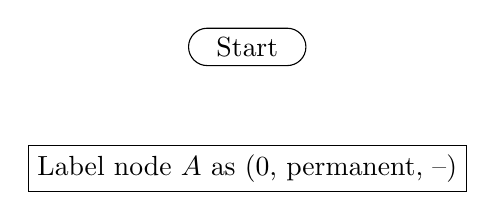
\begin{tikzpicture}
  \label{page:routing:dijkstra:algorithm}

  \node [terminal, draw]  (start) {Start};
  \node [process, draw, below=of start] (markA) {Label node $A$ as (0, permanent, --)}; 
\end{tikzpicture}


\newcommand{\dijkstraGraph}[6]{  \begin{scope}[every node/.style={circle, draw},
    every label/.style={draw=none,font=\small,% yshift=0.5cm,
      align=center},
    label distance=-10pt]
    \node [label=below:{#1 }] (a) {A}; 
    \node [above right=of a, label=below:{#2 }] (b) {B}; 
    \node [above right=of b, label=below:{#3 }] (c) {C};
    \node [right=of c, label=above:{#4}] (d) {D};
    \node [above=of c, label=above:{#5}] (f) {F}; 
    \node [right=of d, label=right:{#6 }] (z) {Z};
  \end{scope}


  \foreach \n/\m/\o/\i/\c/\co  in {a/f/90/180/75/left,
    a/b/45/225/3/above,
    b/f/90/210/4/left,
    b/c/60/210/5/above,
    c/f/90/270/8/right,
    c/d/0/180/10/above,
    d/z/0/180/2/below,
    f/z/0/110/60/above,
    a/z/0/270/150/below,
    b/d/0/270/20/below}
  {
    \draw (\n) to[out=\o,in=\i] node[\co] {\c} (\m); 
  }
}

\begin{tikzpicture}
  \label{page:routing:dijkstra:example:plain}

  \dijkstraGraph{}{}{}{}{}{}
\end{tikzpicture}


\begin{tikzpicture}
  \label{page:routing:dijkstra:example:0}

  \dijkstraGraph{($\infty$, tent., \\unknown)}{($\infty$, tent., \\unknown)}{($\infty$, tent., \\unknown)}{($\infty$, tent., \\unknown)}{($\infty$, tent., \\unknown)}{($\infty$, tent., \\unknown)}
\end{tikzpicture}



\begin{tikzpicture}
  \label{page:routing:dijkstra:example:1}

  \dijkstraGraph{(0, perm., \\--)}{($\infty$, tent., \\unknown)}{($\infty$, tent., \\unknown)}{($\infty$, tent., \\unknown)}{($\infty$, tent., \\unknown)}{($\infty$, tent., \\unknown)}

  % this is totally ugly, but redrawing seems to be the simplest option,
  % lacking proper parameter-passing mechanisms 
  \node [fill=green, circle] at (a) {A}; 
\end{tikzpicture}

\begin{tikzpicture}
  \label{page:routing:dijkstra:example:2}

  \dijkstraGraph{(0, perm., \\--)}{(3, tent., \\A)}{($\infty$, tent., \\unknown)}{($\infty$, tent., \\unknown)}{(75, tent., \\A)}{(15$\infty$, tent., \\A)}

  % this is totally ugly, but redrawing seems to be the simplest option,
  % lacking proper parameter-passing mechanisms 

  \node [fill=green, circle] at (a) {A}; 
  \foreach \n in {b,f,z}
  { \node [fill=hpiyellow, circle] at (\n) {\MakeUppercase \n}; }
   
\end{tikzpicture}

\begin{tikzpicture}
  \label{page:routing:dijkstra:example:3}

  \dijkstraGraph{(0, perm., \\--)}{(3, perm., \\A)}{($\infty$, tent., \\unknown)}{($\infty$, tent., \\unknown)}{(75, tent., \\A)}{(15$\infty$, tent., \\A)}


  % this is totally ugly, but redrawing seems to be the simplest option,
  % lacking proper parameter-passing mechanisms 

  % done: 
  \foreach \done in {a} {
    \node [fill=green!10, circle] at (\done) {\MakeUppercase \done}; 
  }

  % just made permanent
  \node [fill=green, circle] at (b) {B};


  % tentative: 
  \foreach \done in {f,z} {
    \node [fill=hpiorange, circle] at (\done) {\MakeUppercase \done}; 
  }

  
  % now considered 
  \foreach \n in {}
  { \node [fill=hpiyellow, circle] at (\n) {\MakeUppercase \n}; }


  
\end{tikzpicture}

\begin{tikzpicture}
  \label{page:routing:dijkstra:example:4}

  \dijkstraGraph{(0, perm., \\--)}{(3, perm., \\A)}{(8, tent., \\B)}{(23, tent., \\B)}{(7, tent., \\B)}{(15$\infty$, tent., \\A)}


  % this is totally ugly, but redrawing seems to be the simplest option,
  % lacking proper parameter-passing mechanisms 

  % done: 
  \foreach \done in {a} {
    \node [fill=green!10, circle] at (\done) {\MakeUppercase \done}; 
  }

  % just made permanent
  \node [fill=green, circle] at (b) {B};


  % tentative: 
  \foreach \done in {z} {
    \node [fill=hpiorange, circle] at (\done) {\MakeUppercase \done}; 
  }

  
  % now considered 
  \foreach \n in {f, c,d}
  { \node [fill=hpiyellow, circle] at (\n) {\MakeUppercase \n}; }


  
\end{tikzpicture}

\begin{tikzpicture}
  \label{page:routing:dijkstra:example:5}

  \dijkstraGraph{(0, perm., \\--)}{(3, perm., \\A)}{(8, tent., \\B)}{(23, tent., \\B)}{(7, perm., \\B)}{(15$\infty$, tent., \\A)}


  % this is totally ugly, but redrawing seems to be the simplest option,
  % lacking proper parameter-passing mechanisms 

  % done: 
  \foreach \done in {a, b} {
    \node [fill=green!10, circle] at (\done) {\MakeUppercase \done}; 
  }

  % just made permanent
  \node [fill=green, circle] at (f) {F};


  % tentative: 
  \foreach \done in {c, d, z} {
    \node [fill=hpiorange, circle] at (\done) {\MakeUppercase \done}; 
  }

  
  % now considered 
  \foreach \n in {}
  { \node [fill=hpiyellow, circle] at (\n) {\MakeUppercase \n}; }


  
\end{tikzpicture}

\begin{tikzpicture}
  \label{page:routing:dijkstra:example:6}

  \dijkstraGraph{(0, perm., \\--)}{(3, perm., \\A)}{(8, tent., \\B)}{(23, tent., \\B)}{(7, perm., \\B)}{(67, tent., \\F)}


  % this is totally ugly, but redrawing seems to be the simplest option,
  % lacking proper parameter-passing mechanisms 

  % done: 
  \foreach \done in {a, b} {
    \node [fill=green!10, circle] at (\done) {\MakeUppercase \done}; 
  }

  % just made permanent
  \node [fill=green, circle] at (f) {F};


  % tentative: 
  \foreach \done in {d} {
    \node [fill=hpiorange, circle] at (\done) {\MakeUppercase \done}; 
  }

  
  % now considered 
  \foreach \n in {c, z}
  { \node [fill=hpiyellow, circle] at (\n) {\MakeUppercase \n}; }
  
\end{tikzpicture}

\begin{tikzpicture}
  \label{page:routing:dijkstra:example:7}

  \dijkstraGraph{(0, perm., \\--)}{(3, perm., \\A)}{(8, tent., \\B)}{(23, tent., \\B)}{(7, perm., \\B)}{(67, tent., \\F)}


  % this is totally ugly, but redrawing seems to be the simplest optin,
  % lacking proper parameter-passing mechanisms 

  % done: 
  \foreach \done in {a, b, f} {
    \node [fill=green!10, circle] at (\done) {\MakeUppercase \done}; 
  }

  % just made permanent
  \node [fill=green, circle] at (c) {C};


  % tentative: 
  \foreach \done in {d, z} {
    \node [fill=hpiorange, circle] at (\done) {\MakeUppercase \done}; 
  }

  
  % now considered 
  \foreach \n in {}
  { \node [fill=hpiyellow, circle] at (\n) {\MakeUppercase \n}; }
  
\end{tikzpicture}

\begin{tikzpicture}
  \label{page:routing:dijkstra:example:8}

  \dijkstraGraph{(0, perm., \\--)}{(3, perm., \\A)}{(8, perm., \\B)}{(18, tent., \\C)}{(7, perm., \\B)}{(67, tent., \\F)}


  % this is totally ugly, but redrawing seems to be the simplest optin,
  % lacking proper parameter-passing mechanisms 

  % done: 
  \foreach \done in {a, b, f} {
    \node [fill=green!10, circle] at (\done) {\MakeUppercase \done}; 
  }

  % just made permanent
  \node [fill=green, circle] at (c) {C};


  % tentative: 
  \foreach \done in {z} {
    \node [fill=hpiorange, circle] at (\done) {\MakeUppercase \done}; 
  }

  
  % now considered 
  \foreach \n in {d}
  { \node [fill=hpiyellow, circle] at (\n) {\MakeUppercase \n}; }
  
\end{tikzpicture}

\begin{tikzpicture}
  \label{page:routing:dijkstra:example:9}

  \dijkstraGraph{(0, perm., \\--)}{(3, perm., \\A)}{(8, perm., \\B)}{(18, perm., \\C)}{(7, perm., \\B)}{(67, tent., \\F)}


  % this is totally ugly, but redrawing seems to be the simplest optin,
  % lacking proper parameter-passing mechanisms 

  % done: 
  \foreach \done in {a, b, c, f} {
    \node [fill=green!10, circle] at (\done) {\MakeUppercase \done}; 
  }

  % just made permanent
  \node [fill=green, circle] at (d) {D};


  % tentative: 
  \foreach \done in {z} {
    \node [fill=hpiorange, circle] at (\done) {\MakeUppercase \done}; 
  }

  
  % now considered 
  \foreach \n in {}
  { \node [fill=hpiyellow, circle] at (\n) {\MakeUppercase \n}; }
  
\end{tikzpicture}

\begin{tikzpicture}
  \label{page:routing:dijkstra:example:10}

  \dijkstraGraph{(0, perm., \\--)}{(3, perm., \\A)}{(8, perm., \\B)}{(18, perm., \\C)}{(7, perm., \\B)}{(20, tent., \\D)}


  % this is totally ugly, but redrawing seems to be the simplest option,
  % lacking proper parameter-passing mechanisms 

  % done: 
  \foreach \done in {a, b, c, f} {
    \node [fill=green!10, circle] at (\done) {\MakeUppercase \done}; 
  }

  % just made permanent
  \node [fill=green, circle] at (d) {D};


  % tentative: 
  \foreach \done in {} {
    \node [fill=hpiorange, circle] at (\done) {\MakeUppercase \done}; 
  }
  
  
  % now considered 
  \foreach \n in {z}
  { \node [fill=hpiyellow, circle] at (\n) {\MakeUppercase \n}; }
  
\end{tikzpicture}

\begin{tikzpicture}
  \label{page:routing:dijkstra:example:11}

  \dijkstraGraph{(0, perm., \\--)}{(3, perm., \\A)}{(8, perm., \\B)}{(18, perm., \\C)}{(7, perm., \\B)}{(20, perm., \\D)}


  % this is totally ugly, but redrawing seems to be the simplest option,
  % lacking proper parameter-passing mechanisms 

  % done: 
  \foreach \done in {a, b, c, d, f} {
    \node [fill=green!10, circle] at (\done) {\MakeUppercase \done}; 
  }

  % just made permanent
  \node [fill=green, circle] at (z) {Z};


  % tentative: 
  \foreach \done in {} {
    \node [fill=hpiorange, circle] at (\done) {\MakeUppercase \done}; 
  }

  
  % now considered 
  \foreach \n in {}
  { \node [fill=hpiyellow, circle] at (\n) {\MakeUppercase \n}; }
  
\end{tikzpicture}

% \begin{tikzpicture}
%   \label{page:routing:dijkstra:example:6}

%   \dijkstraGraph{(0, perm., \\--)}{(3, perm., \\A)}{(8, perm., \\B)}{(18, tent., \\C)}{(16, perm., \\C)}{(76, tent., \\F)}


%   % this is totally ugly, but redrawing seems to be the simplest optin,
%   % lacking proper parameter-passing mechanisms 

%   % done: 
%   \foreach \done in {a, b, c} {
%     \node [fill=green!10, circle] at (\done) {\MakeUppercase \done}; 
%   }

%   % just made permanent
%   \node [fill=green, circle] at (f) {F};


%   % tentative: 
%   \foreach \done in {d} {
%     \node [fill=hpiorange, circle] at (\done) {\MakeUppercase \done}; 
%   }

  
%   % now considered 
%   \foreach \n in {z}
%   { \node [fill=hpiyellow, circle] at (\n) {\MakeUppercase \n}; }


  
% \end{tikzpicture}

% \begin{tikzpicture}
%   \label{page:routing:dijkstra:example:7}

%   \dijkstraGraph{(0, perm., \\--)}{(3, perm., \\A)}{(8, perm., \\B)}{(18, perm., \\C)}{(16, perm., \\C)}{(2$\infty$, tent., \\D)}


%   % this is totally ugly, but redrawing seems to be the simplest optin,
%   % lacking proper parameter-passing mechanisms 

%   % done: 
%   \foreach \done in {a, b, c, f} {
%     \node [fill=green!10, circle] at (\done) {\MakeUppercase \done}; 
%   }

%   % just made permanent
%   \node [fill=green, circle] at (d) {D};


%   % tentative: 
%   \foreach \done in {} {
%     \node [fill=hpiorange, circle] at (\done) {\MakeUppercase \done}; 
%   }

  
%   % now considered 
%   \foreach \n in {z}
%   { \node [fill=hpiyellow, circle] at (\n) {\MakeUppercase \n}; }


  
% \end{tikzpicture}

% \begin{tikzpicture}
%   \label{page:routing:dijkstra:example:8}

%   \dijkstraGraph{(0, perm., \\--)}{(3, perm., \\A)}{(8, perm., \\B)}{(18, perm., \\C)}{(16, perm., \\C)}{(20, perm., \\D)}


%   % this is totally ugly, but redrawing seems to be the simplest optin,
%   % lacking proper parameter-passing mechanisms 

%   % done: 
%   \foreach \done in {a, b, c, f, d} {
%     \node [fill=green!10, circle] at (\done) {\MakeUppercase \done}; 
%   }

%   % just made permanent
%   \node [fill=green, circle] at (z) {Z};


%   % tentative: 
%   \foreach \done in {} {
%     \node [fill=hpiorange, circle] at (\done) {\MakeUppercase \done}; 
%   }

  
%   % now considered 
%   \foreach \n in {}
%   { \node [fill=hpiyellow, circle] at (\n) {\MakeUppercase \n}; }


  
% \end{tikzpicture}


\begin{tikzpicture}[wordbox/.code={\\\wordbox{1}{#1}}]
  \label{page:routing:dijkstra:flooding}

  \dijkstraGraph{}{}{}{}{}{}

  % packet:
  \begin{scope}[every node/.style={scale=0.75,fill=gray!20}]
    \foreach \n/\o/\fields in {a/left/{B: 3,F: 75,Z: 150},{b/below/{A: 3,F: 4,C: 5,D: 20}},{z/right/{D: 2,A: 150, F: 60}},{d/above/{C: 10, B: 20, Z: 2}},{f/left/{A: 75,B: 4,C: 8,Z: 60}},{c/below right/{B: 5,D: 10,F: 8}}}{
      \node [\o=0.1cm of \n] {
        \begin{bytefield}{8}
          \wordbox{1}{Src: \MakeUppercase \n}  
          \\ \wordbox{1}{Seq. num.}
          % expand once based on https://tex.stackexchange.com/questions/680093/using-foreach-to-add-variable-number-of-rows-to-a-bytefield-inside-a-tikz-node
          \tikzset{wordbox/.list/.expand once=\fields}
        \end{bytefield}
      }; 
      }
    
    
  % \node [left=0.1cm of a] {
  %   \begin{bytefield}{8}
  %     \wordbox{1}{Src: A} \\
  %     \wordbox{1}{Seq. num.} \\
  %     \bitbox{4}{B} & \bitbox{4}{3} \\
  %     \bitbox{4}{F} & \bitbox{4}{75} \\
  %     \bitbox{4}{Z} & \bitbox{4}{150} \\
  %   \end{bytefield}};
    
  \end{scope}

  
  
\end{tikzpicture}



\end{document} 